\section{Softwarearkitektur}

\subsection{Applikationsmodel}

Applikationsmodellen er valgt ud fra udviklernes synspunkt og bruges for at give overblik over hvilke klasser som skal laves, og hvilket ansvar de hver især har. Nedenstående UML skal ses som det overordnede system og menuklasserne er udeladt for at skabe overblik. 

\begin{figure}[!h]
\centering 
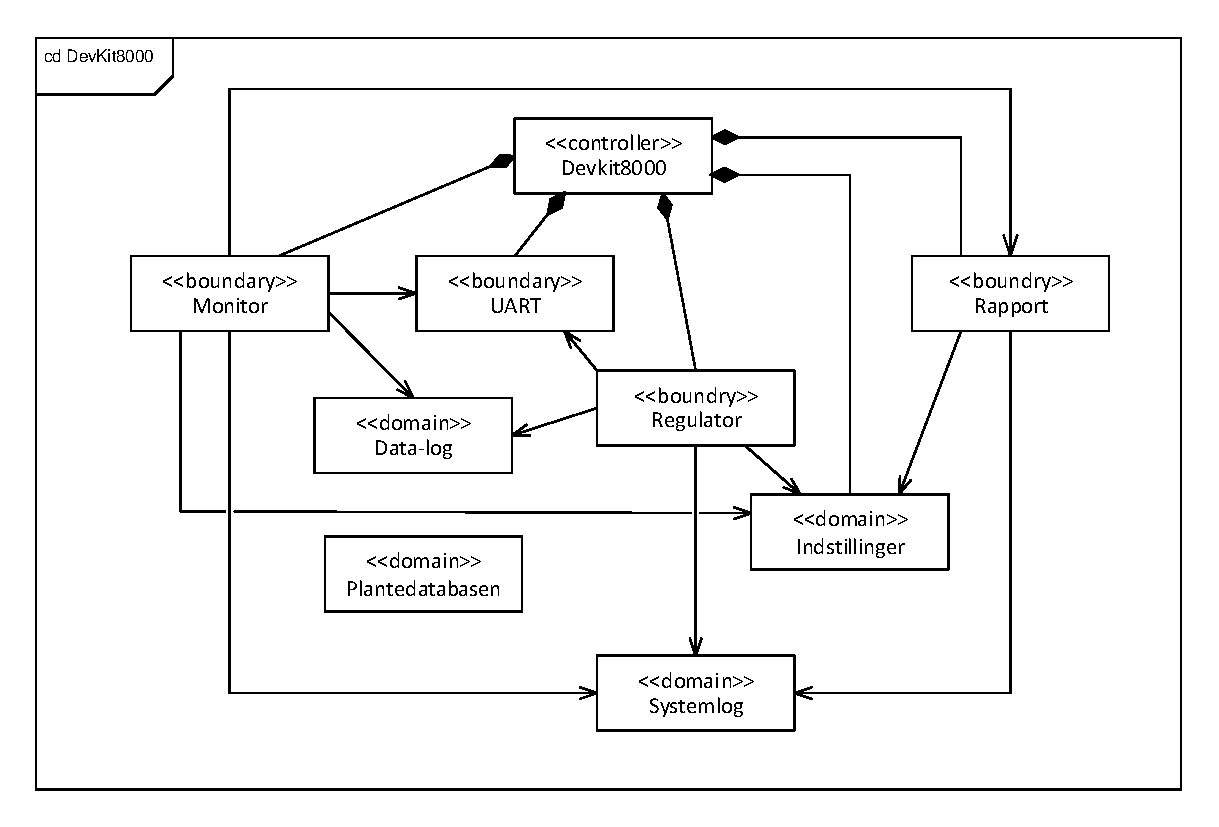
\includegraphics[scale=0.8] {../fig/UML_autogreen.pdf}
\caption{Application model for AutoGreen}
\label{fig:UML}
\end{figure}

\subsection{Controller-Klasser}

\subsubsection{DevKit8000}

DevKit8000 klassen skal initiere systemet og har derfter ansvaret for styring af processerne Regulering og Monitoring.
DevKit8000 klassen indeholder alle menuer beskrevet i menuoversigt. Brugeren kan interagere med klassen igennem menuerne.
Controller-klassen har igennem menuerne set i menuoversigten tilgang til de andre klasser i systemet.

\subsection{Boundary-Klasser}

\subsubsection{Monitor}

Monitorklassens primære opgave er at opsamle sensordata fra UART klassen og skrive dem til data-loggen. Der ud over skal Monitor skrive til System-log, hvis UART klassen rapporterer fejl ved dataoverførelse.

\subsubsection{Regulator}

Reguleringsklassen har ansvaret for at planterværdierne bliver overholdt. Den opnår dette ved at læse fra data-loggen og hvis uregelmæssigheder findes blandt disse data, vil klassen tænde de fornødende akutuatorer gennem UART klassen. Der ud over skal Regulator skrive til System-log, hvis UART klassen rapporter fejl ved data overførelse.

\subsubsection{UART}

UARTklassen er grænsefladen mellem Devkittet og de sensorer/akutuatorer, der måtte eksistere i AutoGreen systemet.

\subsubsection{Rapport}

Rapportering indlæser E-mailkonfigurationer fra indstillinger, som bestemmer hvilke funktionaliteter, der skal benyttes. Rapporting skal sende E-mail til brugeren dagligt, når der er kritisk klima i drivhuset, eller både dagligt og ved kritisk klima. 

\subsection{Domain-Klasser}

\subsubsection{Data-log}

Data-loggen styrer en datastruktur. Det er dens opgave at modtage og indsætte målte data from drivhusklima i datastrukturen, samt hente informationer ud fra strukturen.

\subsubsection{System-log}

System-loggen har til ansvar at styre en datastruktur med henblik på at gemme de vigtigste systemhændelser og skal kunne tilgåes af brugeren senere.

\subsubsection{Indstillinger}

Indstillinger gemmer konfigurationer og indlæser dem i konfigurationsfilen, når regulering eller rapportering startes af brugeren. 

\subsubsection{Plantedatabasen}

Plantedatabasen gemmer parametre for brugerdefinerede planter samt  prækonfigurede planter og tilgås via en klasse menu.

\clearpage

\subsection{Menuoversigt}

Menuoversigten giver et overblik over de forskellige menuer og hvilke menuer, der giver tilgang til hinanden.

\begin{figure}[!h]
\centering 
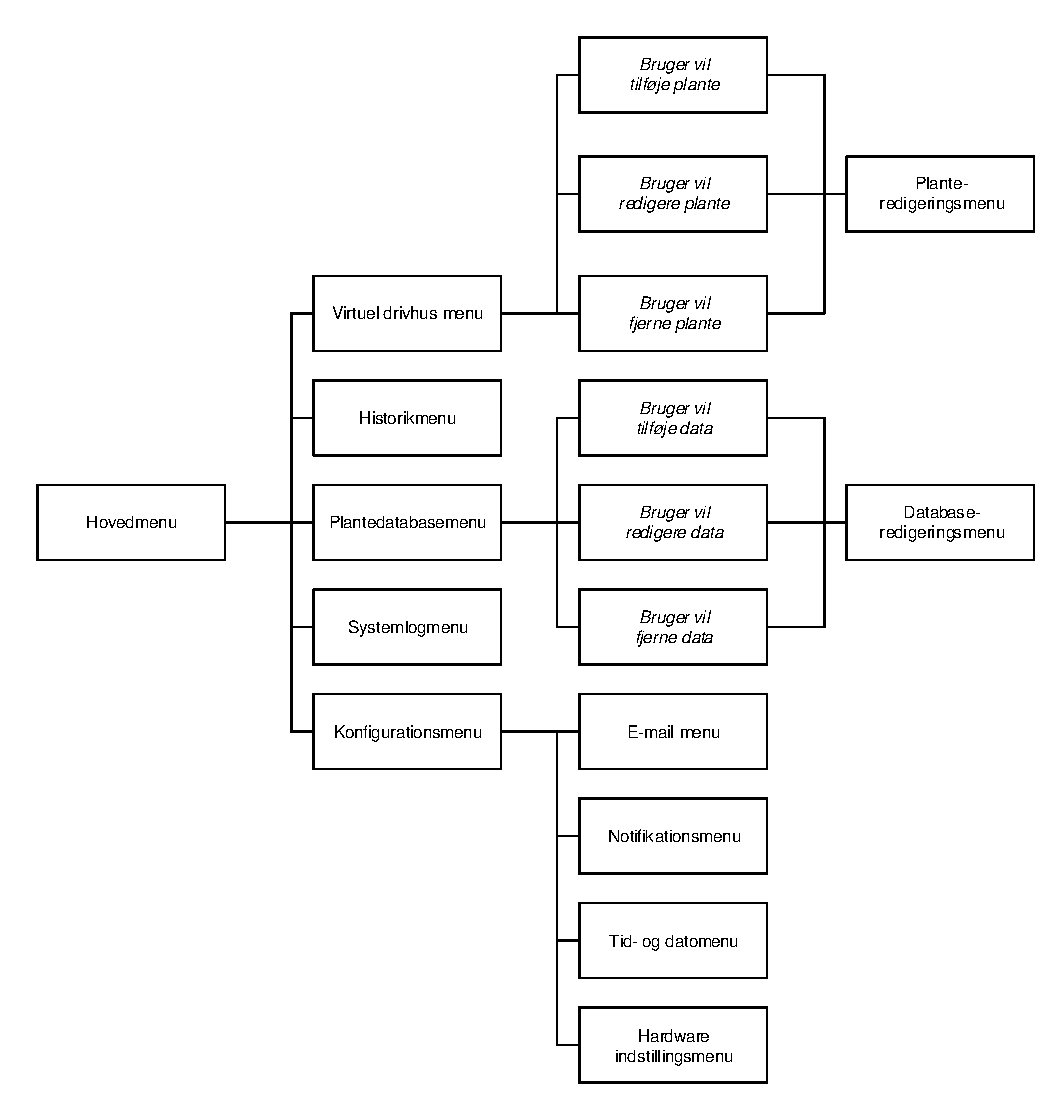
\includegraphics[scale=0.7] {../fig/menu_oversigt.pdf}
\caption{Oversigt over AutoGreen's menuer}
\label{fig:QTMenu}
\end{figure}

\subsection{Menubeskrivelse}
Menuoversigten er med til at give et overblik over hvordan de forskellige menuer tilgåes igennem systemet, og fra hvilke menuer man kan tilgå andre menuer. Hovedmenuen er som standard stedet, hvor brugeren starter, da er her muligt at monitorere drivhusklimaet. I hovedmenuen har brugeren mulighed for at tilgå de 5 undermenuer: virtuel drivhus-, historik-, plantedatabase-, systemlog- og konfigurationsmenu.

\subsubsection{Virtuelle drivhusmenu}
I det virtuelle drivhus har brugeren mulighed for at tilføje nye planter til drivhuset, redigere allerede tilstedeværende planter, og herunder slette planter fra drivhuset. Uanset ønsket skal brugeren tilgå planteredigeringsmenuen.

\subsubsection{Historikmenu}
I historikmenuen har brugeren mulighed for at se data over drivhuset op til et år tilbage.

\subsubsection{Plantedatabasemenu}
I plantedatabasemenuen har brugeren mulighed for at tilføje nye planter til databasen. Ved tryk på 'tilføj plante' oprettes en ny tom virtuel plante i databasen. Denne virtuelle plante åbnes i databaseredigeringsmenuen, hvor dens paramentre kan indstilles efter behov. Hvis brugeren ønsker at redigere allerede oprettede planter eller slette disse, kan brugeren trykke på den ønskede plante. Den valgte plante vil blive åbnet gennem databaseredigeringsmenuen, og det er her muligt at redigere eller slette planten.

\subsubsection{Systemlogmenu}
I systemloggen har brugeren mulighed for at se systemhændelser, f.eks. hvis systemet vælger at åbne et vindue, starte en blæser, eller bruge varmelegemet.

\subsubsection{Konfigurationsmenu}
I konfigurationsmenu har brugeren mulighed for at tilgå 4 undermenuer: E-mailmenu, Notifikationsmenu, Tid- og datomenu, samt Hardware Indstillingsmenu.

\subsubsection{E-mailmenu}
I E-mailmenuen, vises 3 kolonner, hvor brugeren har mulighed for at indtaste E-mail adresse, som skal modtage notifiktationer. 

\subsubsection{Notifikationsmenu} 
I notifikationsmenuen har brugeren mulighed for at slå notifikationer til og fra for både advarsels-notifikationer og daglige notifikationer. 

\subsubsection{Tids- og datomenu} 
I Tids- og datomenuen har brugeren mulighed for at ændre dato og tid. 

\subsubsection{Hardware Indstillingsmenu} 
I Hardware Indstillingsmenu har brugeren mulighed for at vælge hvilke akutuatorer drivhuset skal bruge. Hvis brugeren ønsker at spare strøm, kan blæser og varmelegeme fravælges til regulering temperaturen. \\
